\documentclass{article}

\usepackage{mathptmx}
%packages for language
\usepackage[czech]{babel}
\usepackage[utf8]{inputenc}
%packages for graphic
\usepackage{graphicx}
\usepackage{pgfplots}
\usepackage{pgfplotstable}
\usepackage{multirow}
\usepackage{tikz}
\usepackage{import}
\usepackage[a4paper, total={17cm,25.7cm}, top=2cm, left=2cm, includefoot]{geometry}
\usepackage{todonotes}
\usepackage{standalone}
\usepackage{colortbl}%pro barevne zmeny v tabulce
\usepackage{float}
\usepackage{csvsimple} %pro import a práci s csv soubory
\usepackage{indentfirst}  % odsazení prvního řádku v odstavci
\usepackage{hyperref} %dela odkazy na mista v dokumentu atd
\usepackage{amsmath}%psani matic
\usepackage{mathrsfs}%psani kroucenym matematickym pismem
\usepackage{pdfpages}%vkladani celych pdf dokumentu
%cesta k obrazkum: ./Graphics/....

\begin{document}
	\begin{titlepage}
    \begin{center}
        \LARGE
        Západočeská Univerzita v Plzni\\
        Fakulta Aplikovaných Věd\\
        
        \vspace{1cm}
        
        
\includegraphics[width=0.5\textwidth]{./Graphics/FAV_logo.pdf}
        
        \vspace{4cm}
        
        \textbf{Semestrální práce z předmětu KKY/SYA}\\
        Databáze osobního účetnictví
        
        \vspace{0.5cm}
        Filip Jašek
        
    \end{center} 
    \vfill
        \noindent
        \large
        Předmět: KKY/SYA (Systémová analýza)\\
        Přednášející: Ing. Václav Hajšman, Ph.D.\\
        Cvičící: Ing. Miloš Fetter\hfill Datum: \today
\end{titlepage}
	
	
	\section{Motivace}
	Jelikož se jako student nechávám často zaměstnávat na tzv. DPP a během jednoho roku mohu pracovat souběžně ve více firmách najednou, musím odvádět daně ze smluv, kde nemám podepsáno daňové prohlášení. Věřím, že nejsem jediný student, co takto pracuje a proto jsem se rozhodl vytvořit jednoduchou databázi, která je určena pro správu osobního účetnictví. Výrazně zjednodušuje orientaci v podepsaných smlouvách, vykonaných pracích a jednotlivých výplatách, díky čemuž by mohla usnadnit podání daňového přiznání.
	
	\section{Představení}
	Databáze byla vytvořena v programu Microsoft Access, kvůli jeho přívětivosti pro začátečníky a možnosti vytvořit základní grafické rozhraní pro zadávání dat.
	\begin{figure}[H]
		\centering
		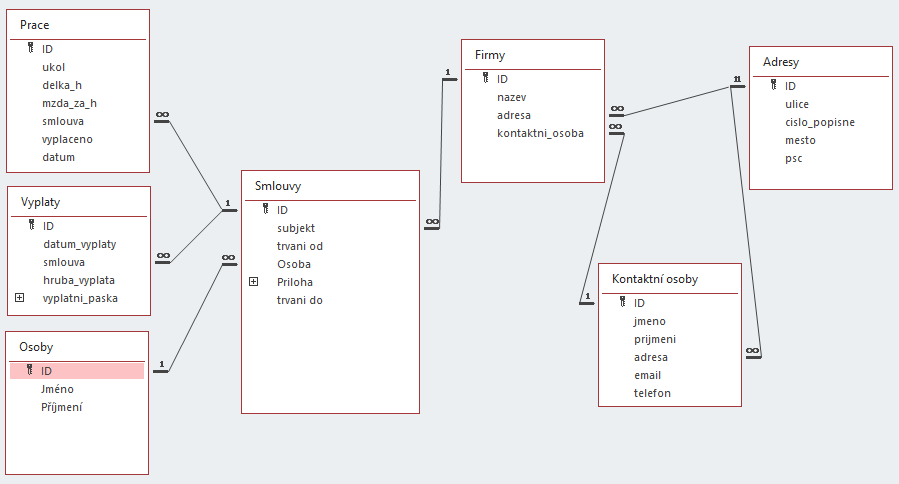
\includegraphics[width=\textwidth]{./Graphics/relace}
		\caption{Relace jednotlivých tabulek v databázi.}
		\label{pic:relace}
	\end{figure}
	Jak lze vidět z Obrázku \ref{pic:relace}, databáze se skládá ze sedmi tabulek. Každá má svou speciální funkci a jejich obsah může být do budoucna rozšířen o další pole. Jednotlivé tabulky mají odlišné důvody existence, které jsou popsány níže.\\
	\textbf{Osoby}\\
	- tabulka obsahující jednotlivé uživatele, ke kterým se vážou zaznamenané smlouvy\\
	\textbf{Smlouvy}\\
	- obsahuje reálné existující smlouvy, které se vážou na jednotlivé osoby\\
	- kromě dat uvedených na smlouvě v papírové podobě na sebe váže i informace o výplatách a vykonaných pracích.\\
	\textbf{Firmy}\\
	- sdružuje data o jednotlivých subjektech uvedených ve smlouvách jako zaměstnavatel\\
	\textbf{Kontaktní osoby}\\
	- osoby s jistou vazbou na firmu, na které se lze obrátit s nejasnostmi ve smlouvě\\
	- obsahuje kontaktní informace na dané osoby\\
	\textbf{Adresy}\\
	- tabulka adres s vazbou na \textbf{Firmy} a \textbf{Kontaktní osoby}\\
	\textbf{Práce}\\
	- seznam prací s vazbou na smlouvy a informacemi o práci, délce práce, mzdy, datum a datum vyplacení\\
	\textbf{Výplaty}\\
	- záznamy jednotlivých výplat včetně informace o zaplacených pracích a výši hrubé výplaty\\
	
	\section{Obsluha}
	Vstupní branou do databáze je "Hlavní formulář" (Obrázek \ref{pic:hlavni_formular}), který obsahuje nejdůležitější odkazy na zadání nové smlouvy a práce v podobě zelených tlačítek a odkazy pro správu již zadaných informací.
	
	\begin{figure}[H]
		\centering
		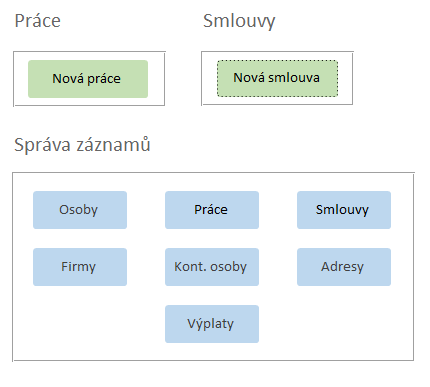
\includegraphics[width=.5\textwidth]{./Graphics/hlavni_formular}
		\caption{Vstupní brána do databáze v podobě Hlavního formuláře.}
		\label{pic:hlavni_formular}
	\end{figure}
	Pro zadání nové práce je však podstatné mít již zaznamenanou osobu, smlouvy a další související informace.
	

	\section{Závěr}
	Databáze funguje tak, jak byla zamýšlena a určitě má potenciál reálného využití, jak pro studenty, tak pro živnostníky a nebo pro zpřehlednění výkazů v malých firmách v rámci digitalizace účetnictví. Měřit se s již existujícími systémy pro správu účetnictví nemůže, ale nenáročný úkol zpřehlednit ho splnit dokáže. Jako rozšíření by se daly přidat výpočty čisté mzdy, kolik ze mzdy je sociální a zdravotní pojištění nebo jiné potřebné údaje pro záznam do daňového přiznání.
	
\end{document}
